\documentclass[11pt, letterpaper]{article}
\usepackage[utf8]{inputenc}
\usepackage[letterpaper, margin=0.5in]{geometry}
\usepackage{amsmath}
\usepackage{amssymb}
\usepackage{amsthm}
\usepackage{graphicx}
\usepackage{listings}
\usepackage[font=scriptsize]{caption}
\usepackage{subcaption}
\usepackage{xcolor}

\definecolor{codegreen}{rgb}{0,0.6,0}
\definecolor{codegray}{rgb}{0.5,0.5,0.5}
\definecolor{codepurple}{rgb}{0.58,0,0.82}
\definecolor{backcolour}{rgb}{0.95,0.95,0.92}

\lstdefinestyle{mystyle}{
    backgroundcolor=\color{backcolour},   
    commentstyle=\color{codegreen},
    keywordstyle=\color{magenta},
    numberstyle=\tiny\color{codegray},
    stringstyle=\color{codepurple},
    basicstyle=\ttfamily\footnotesize,
    breakatwhitespace=false,
    texcl=true,
    mathescape=true,
    breaklines=true,                 
    captionpos=b,                    
    keepspaces=true,                 
    numbers=left,                    
    numbersep=5pt,                  
    showspaces=false,                
    showstringspaces=false,
    showtabs=false,                  
    tabsize=2
}

\lstset{style=mystyle}
\graphicspath{ {.} }
\captionsetup{justification=raggedright, singlelinecheck=false}

\author{Ryan Tang}
\title{STA 602 HW 11}
\date{November 18th 2022}

\begin{document}
\maketitle

\section{Exercise 8.1}
\paragraph{(a)}
$Var[y_{i,j}|\mu, \tau^2]$ should be bigger than $Var[y_{i,j}|\theta_j, \sigma^2]$ that the variances of the population should always be larger or equal to the with-in group variances. The worse case is that the two variances are the same, $\theta_i=\mu \, \forall i$.

\paragraph{(b)}
$Cov[y_{i_1,j}, y_{i_2, j}|\theta_j, \sigma^2]$ should be closer to zero under the conditional iid assumption from the model. In other words, other observations in the same group don't tell us additional information if we already know the group's average performance.

$Cov[y_{i_1,j}, y_{i_2, j}|\mu, \tau^2]$ should be either negative or positive when the group-specific performance is unknown. The sign has to be determined by the actual observation differences and $\tau^2$. If the two observation is far-part, then we think it gives us some information that the group means should be in the middle of the two --- negative covariance. On the other hand, if the two observations are close, the group means will shrink towards the global mean $\mu$ --- positive covariance.

\paragraph{(c)}
Following the conditional independence of the hierarchical model, we have the following. We can see the population variances are always higher than the within-group variances by $\tau^2$.
\begin{align*}
    Var[y_{i,j}|\theta_j, \sigma^2] &= \sigma^2 \\
    Var[y_{i,j}|\mu, \tau^2] &= \mathbb{E}[Var[y_{i,j}|\theta_j, \sigma^2]|\mu, \tau^2] + Var[\mathbb{E}[y_{i,j}|\theta_j, \sigma^2]|\mu, \tau^2] \\
        &= \mathbb{E}[\sigma^2] + Var[\sigma_j|\mu, \tau^2] \\
        &= \sigma^2 + \tau^2 \\
    Var[\bar{y}_{.,j}|\theta_j, \sigma^2] &= \frac{1}{N_j^2} Var[\sum_i y_{i,j}|\theta_j, \sigma^2] \\
        &= \frac{\sigma^2}{N_j} \\
    Var[\bar{y}_{.,j}|\mu, \tau^2]
        &= \mathbb{E}[\frac{1}{N_j^2} Var[y_{i,j}|\theta_j \sigma^2]|\mu, \tau^2] + Var[\frac{1}{N_j} \mathbb{E}[y_{i,j}|\theta_j]|\mu, \tau^2] \\
        &= \mathbb{E}[\frac{\sigma^2}{N_j}|\mu, \tau^2] + Var[\theta_j|\mu, \tau^2] \\
        &= \frac{m}{N} \sigma^2 + \tau^2 \\
    Cov[y_{i_1, j}, y_{i_2, j}|\theta_j, \sigma^2]
        &= \mathbb{E}[y_{i_1, j}, y_{i_2, j}|\theta_j, \sigma^2] - \mathbb{E}[y_{i, j}|\theta_j, \sigma^2]\mathbb{E}[y_{i, j}|\theta_j, \sigma^2] \\
        &= Var[y_{i,j}|\theta_j, \sigma^2] \\
        &= \sigma^2 \\
    Cov[y_{i_1, j}, y_{i_2, j}|\theta_j, \sigma^2] &= Var[y_{i,j}|\mu, \tau^2] \\
        &= \sigma^2 + \tau^2
\end{align*}

\paragraph{(d)}
In words, the posterior of the population mean depends only on the posterior within group means. Of course, the with-in group posterior means have already incorporated all the information from the individual data points.
\begin{align*}
    p(\mu|\theta, \sigma^2, \tau^2, Y) &\propto p(\mu) p(\theta|\mu, \tau^2) p(Y|\theta, \sigma^2) \\
        &\propto p(\mu) p(\theta|\mu, \tau^2) \\
        &\propto p(\theta, \mu|\tau^2) \\
        &= p(\mu|\theta, \tau^2)
\end{align*}


\section{Exercise 8.2}
We are given the following hierarchical model.
\begin{align*}
    \theta_A &= \mu + \delta \\
    \theta_B &= \mu - \delta \\
    \mu &\thicksim \mathcal{N}(\mu_o=75, \lambda_o^2=100=\tilde{\lambda}_o^{-1}) \\
    \delta &\thicksim \mathcal{N}(\delta_o, \tau_o^2=\tilde{\tau}_o^{-1}) \\
    \gamma &= \frac{1}{\sigma^2} \thicksim Gamma(\nu_o=1, \sigma_o^2=100) \\
    y_i &\thicksim \mathcal{N}(\mu, \delta, \sigma^2) \\
\end{align*}
The full conditionals for all the parameters $\mu, \gamma, \delta$ are given below.
\begin{align*}
    N_A &= \sum_i^N \mathbb{I}(y_i \in A) \\
    N_B &= \sum_i^N \mathbb{I}(y_i \in B) \\
    N &= N_A + N_B \\
    p(\delta|\mu, Y, \sigma^2)
        &= p(\delta) \prod_i^{N_A} \mathcal{N}(y_{A_i}|\mu+\delta, \sigma^2) \prod_i^{N_B} \mathcal{N}(y_{B_i}|\mu-\delta, \sigma^2) \\
        &\thicksim \mathcal{N} (
            \delta_n=\tau_n^2[\tilde{\tau}_o\delta_o + \gamma(N_A\bar{\tilde{Y}}_A + N_B\bar{\tilde{Y}}_B)],
            \tau_n^2=(\tilde{\tau}_o + \gamma N)^{-1}
        ) \\
    \bar{Y}_{A,\delta} &= \frac{1}{N_A} \sum_{i\in A} (y_i - \mu) \quad \bar{Y}_{B,\delta} = \frac{1}{N_B} \sum_{i\in B} (\mu - y_i) \\ \\
    p(\mu|\delta, Y, \sigma^2)
        &\thicksim \mathcal{N} (
            \delta_n=\lambda_n^2[\tilde{\lambda}_o\delta_o + \gamma(N_A\bar{\tilde{Y}}_A + N_B\bar{\tilde{Y}}_B)],
            \lambda_n^2=(\tilde{\lambda}_o + \gamma N)^{-1}
        ) \\
    \bar{Y}_{A,\mu} &= \frac{1}{N_A} \sum_{i\in A} (y_i - \delta) \quad \bar{Y}_{B,\mu} = \frac{1}{N_B} \sum_{i\in B} (y_i + \delta) \\ \\
    p(\gamma|\delta, \mu, Y)
        &\thicksim Gamma(
            \nu_u = \nu_0+N,
            \sigma_n^2 = \frac{1}{\nu_n} (
                \nu_o\sigma_o^2
                + \sum_{i\in A} (y_{A_i} - \mu - \delta)^2
                + \sum_{i\in B} (y_{B_i} - \mu + \delta)^2
            )
        ) \\
\end{align*}

\paragraph{(a) Sensitivity Analysis}
Below are the posterior results from a wide range of different combinations of prior parameters. All chains behave quite nicely after 1000 burn-in periods. And all statistics were calculated using 10,000 MCMC samples.
\begin{itemize}
    \item We are certainly seeing some evidence that $\delta$ is negative, the mean of group A is greater than group B.
    \item We see that larger prior variances, $\tau_o$, leads to a higher probability that $\theta_B$ is less than $\theta_A$ when $\delta_0$ is positive. However, it also contributes to a wider confidence interval because we only have 32 observations. Posterior correlation also shrinks towards 0 when we have higher variance priors
\end{itemize}

\begin{tabular}{||c c || c c c c c||}
    \hline
    $\delta_o$ & $\tau^2_0$ & $P[\delta < 0|Y]$	& 95\% CI LB & 95\% CI UB & Post Theta Corr & Prior Theta Corr \\
    \hline \hline
    -4 & 10 & 0.88 & -7.83 & 2.01 & 0.40 & 0.82 \\
    \hline
    -4 & 50 & 0.70 & -8.74 & 4.85 & 0.08 & 0.33 \\
    \hline
    -4 & 100 & 0.66 & -9.03 & 5.85 & 0.01 & 0.01 \\
    \hline
    -4 & 500 & 0.62 & -9.42 & 6.75 & -0.06 & -0.67 \\
    \hline
    -2 & 10 & 0.75 & -6.53 & 3.20 & 0.40 & 0.82 \\
    \hline
    -2 & 50 & 0.66 & -8.39 & 5.56 & 0.07 & 0.33 \\
    \hline
    -2 & 100 & 0.63 & -8.82 & 6.23 & 0.00 & -0.01 \\
    \hline
    -2 & 500 & 0.62 & -9.15 & 6.86 & -0.07 & -0.67 \\
    \hline
    0 & 10 & 0.57 & -5.27 & 4.50 & 0.40 & 0.82 \\
    \hline
    0 & 50 & 0.59 & -7.78 & 6.05 & 0.07 & 0.33 \\
    \hline
    0 & 100 & 0.60 & -8.47 & 6.48 & 0.00 & 0.00 \\ 
    \hline
    0 & 500 & 0.61 & -8.80 & 7.00 & -0.05 & -0.67 \\
    \hline
    2 & 10 & 0.38 & -3.96 & 5.68 & 0.40 & 0.82 \\
    \hline
    2 & 50 & 0.54 & -7.32 & 6.68 & 0.05 & 0.34 \\
    \hline
    2 & 100 & 0.58 & -8.09 & 6.73 & -0.01 & 0.00 \\
    \hline
    2 & 500 & 0.60 & -9.10 & 6.64 & -0.05 & -0.67 \\
    \hline
    4 & 10 & 0.21 & -2.85 & 6.92 & 0.41 & 0.82 \\
    \hline
    4 & 50 & 0.49 & -6.93 & 7.24 & 0.06 & 0.33 \\ 
    \hline
    4 & 100 & 0.54 & -7.81 & 7.20 & -0.00 & -0.01 \\
    \hline
    4 & 500 & 0.59 & -8.89 & 7.05 & -0.07 & -0.67 \\
    \hline

\end{tabular}


\paragraph{(b) Prior Opinions}
\begin{itemize}
    \item If one has no strong opinion or belief $\tau^2_o=500$, she can use a diffuse prior with $\delta=0$. In this case, $P[\delta<0|Y] = 0.61$ with a wide 95\% confidence interval. In other words, she will need more evidence to confirm the differences.
    \item If one is sure that Group A under-performs Group B on average but uncertain about the truthfulness of this belief, she can opt for a $\delta_o=-4, \, \tau^2_o=500$ prior. It, too, leads to a $p[\delta<0|Y] = 0.62$ and a wide 95\% confidence interval.
    \item One can also be strongly confident that Group A under-performs Group B; she can choose a $\delta_o=-4, \, \tau_o^2=10$ prior.
    \item One can also use unit information prior, which corresponds to $\delta_o=-2, \, \tau_0^2=50$.
\end{itemize}



\section{Exercise 8.3}
We are given data from 8 schools and would like to use the hierarchical normal model to do inference among schools.
\begin{align*}
    y_{ij}|\theta_j, \sigma^2 &\thicksim \mathcal{N}(y_{ij}|\theta_j, \sigma^2) && i = 1\dots N, \, j = 1\dots M \\
    \theta_j|\mu, \tau^2 &\thicksim \mathcal{N}(\theta_j|\mu, \tau^2) \\
    \mu &\thicksim \mathcal{N}(\mu|\mu_o, \gamma_o^2) \\
    \frac{1}{\tau^2} &\thicksim Gamma(\eta_o, \tau_o^2) \\
    \frac{1}{\sigma^2} &\thicksim Gamma(\nu_o, \sigma^2_o) \\
\end{align*}

And the posterior full conditionals are given below.
\begin{align*}
    \theta_j|Y, \mu, \tau^2, \sigma^2
        &\propto p(\theta_j|\mu, \tau^2) p(y_{.j}|\theta_j, \sigma^2) \\
        &\propto p(\theta_j|\mu, \tau^2) \prod_i^{n_j} p(y_{ij}|\theta_j, \sigma^2) \\
        &\thicksim \mathcal{N} \left[\theta_j |
            \mu_n = \tau^2_n (\frac{1}{\sigma^2}n_j \bar{y}_j + \frac{1}{\tau^2} \mu),
            \tau^2_n = (\frac{1}{\sigma^2} n_j + \frac{1}{\tau^2})^{-1}
        \right] \\ \\
    \mu|Y, \tau^2, \theta
        &\propto \left[ \prod_j^m p(\theta_j|\mu, \tau^2) \right] p(\mu|\mu_o, \gamma^2_o) \\
        &\thicksim \mathcal{N} \left[ \mu|
            \mu_n = \gamma^2_n(\frac{1}{\tau^2}m\bar{\theta} + \frac{1}{\gamma^2_o} \mu_o),
            \gamma^2_n = (\frac{1}{\tau^2} m + \frac{1}{\gamma^2_o})^{-1}
        \right] \\ \\
    \frac{1}{\tau^2}|Y, \mu, \theta
        &\propto p(\tau^2|\eta_o, \tau_o^2) \prod_j^m p(\theta_j|\mu, \tau^2) \\
        &\thicksim Gamma \left[ \alpha=\frac{m+\eta_o}{2}, \beta=\frac{1}{2}(\eta_o\tau_o^2 + \sum_j(\theta_j - \mu)^2) \right] \\ \\
    \frac{1}{\sigma^2}|Y, \theta_
        &\propto p(\sigma^2|\nu_o, \sigma^2_o) \prod_j^m \prod_i^{n_j} p(y_{ij}|\theta_j, \sigma^2) \\
        &\thicksim Gamma \left[ \alpha=\frac{n+\nu_o}{2}, \beta=\frac{1}{2}(\nu_o\sigma_o^2 + \sum_j\sum_i(y_{ij} - \theta_j)^2) \right] \\ \\
\end{align*}

\paragraph{(a) Gibbs Sampling}
Using the above full conditionals, I drew 10,000 MCMC samples after a 1,000 burn-in period. Below is the trace plots, auto-correlation plots, and the corresponding density plots for each variable. We can see the chains perform just fine with good mixing and converges quite succesfully.
\begin{itemize}
    \item ESS for $\sigma^2$ is 8,995
    \item ESS for $\tau^2$ is 9,551
    \item ESS for $\mu$ is 5,948
\end{itemize}
\begin{figure*}[!h]
  \centering
  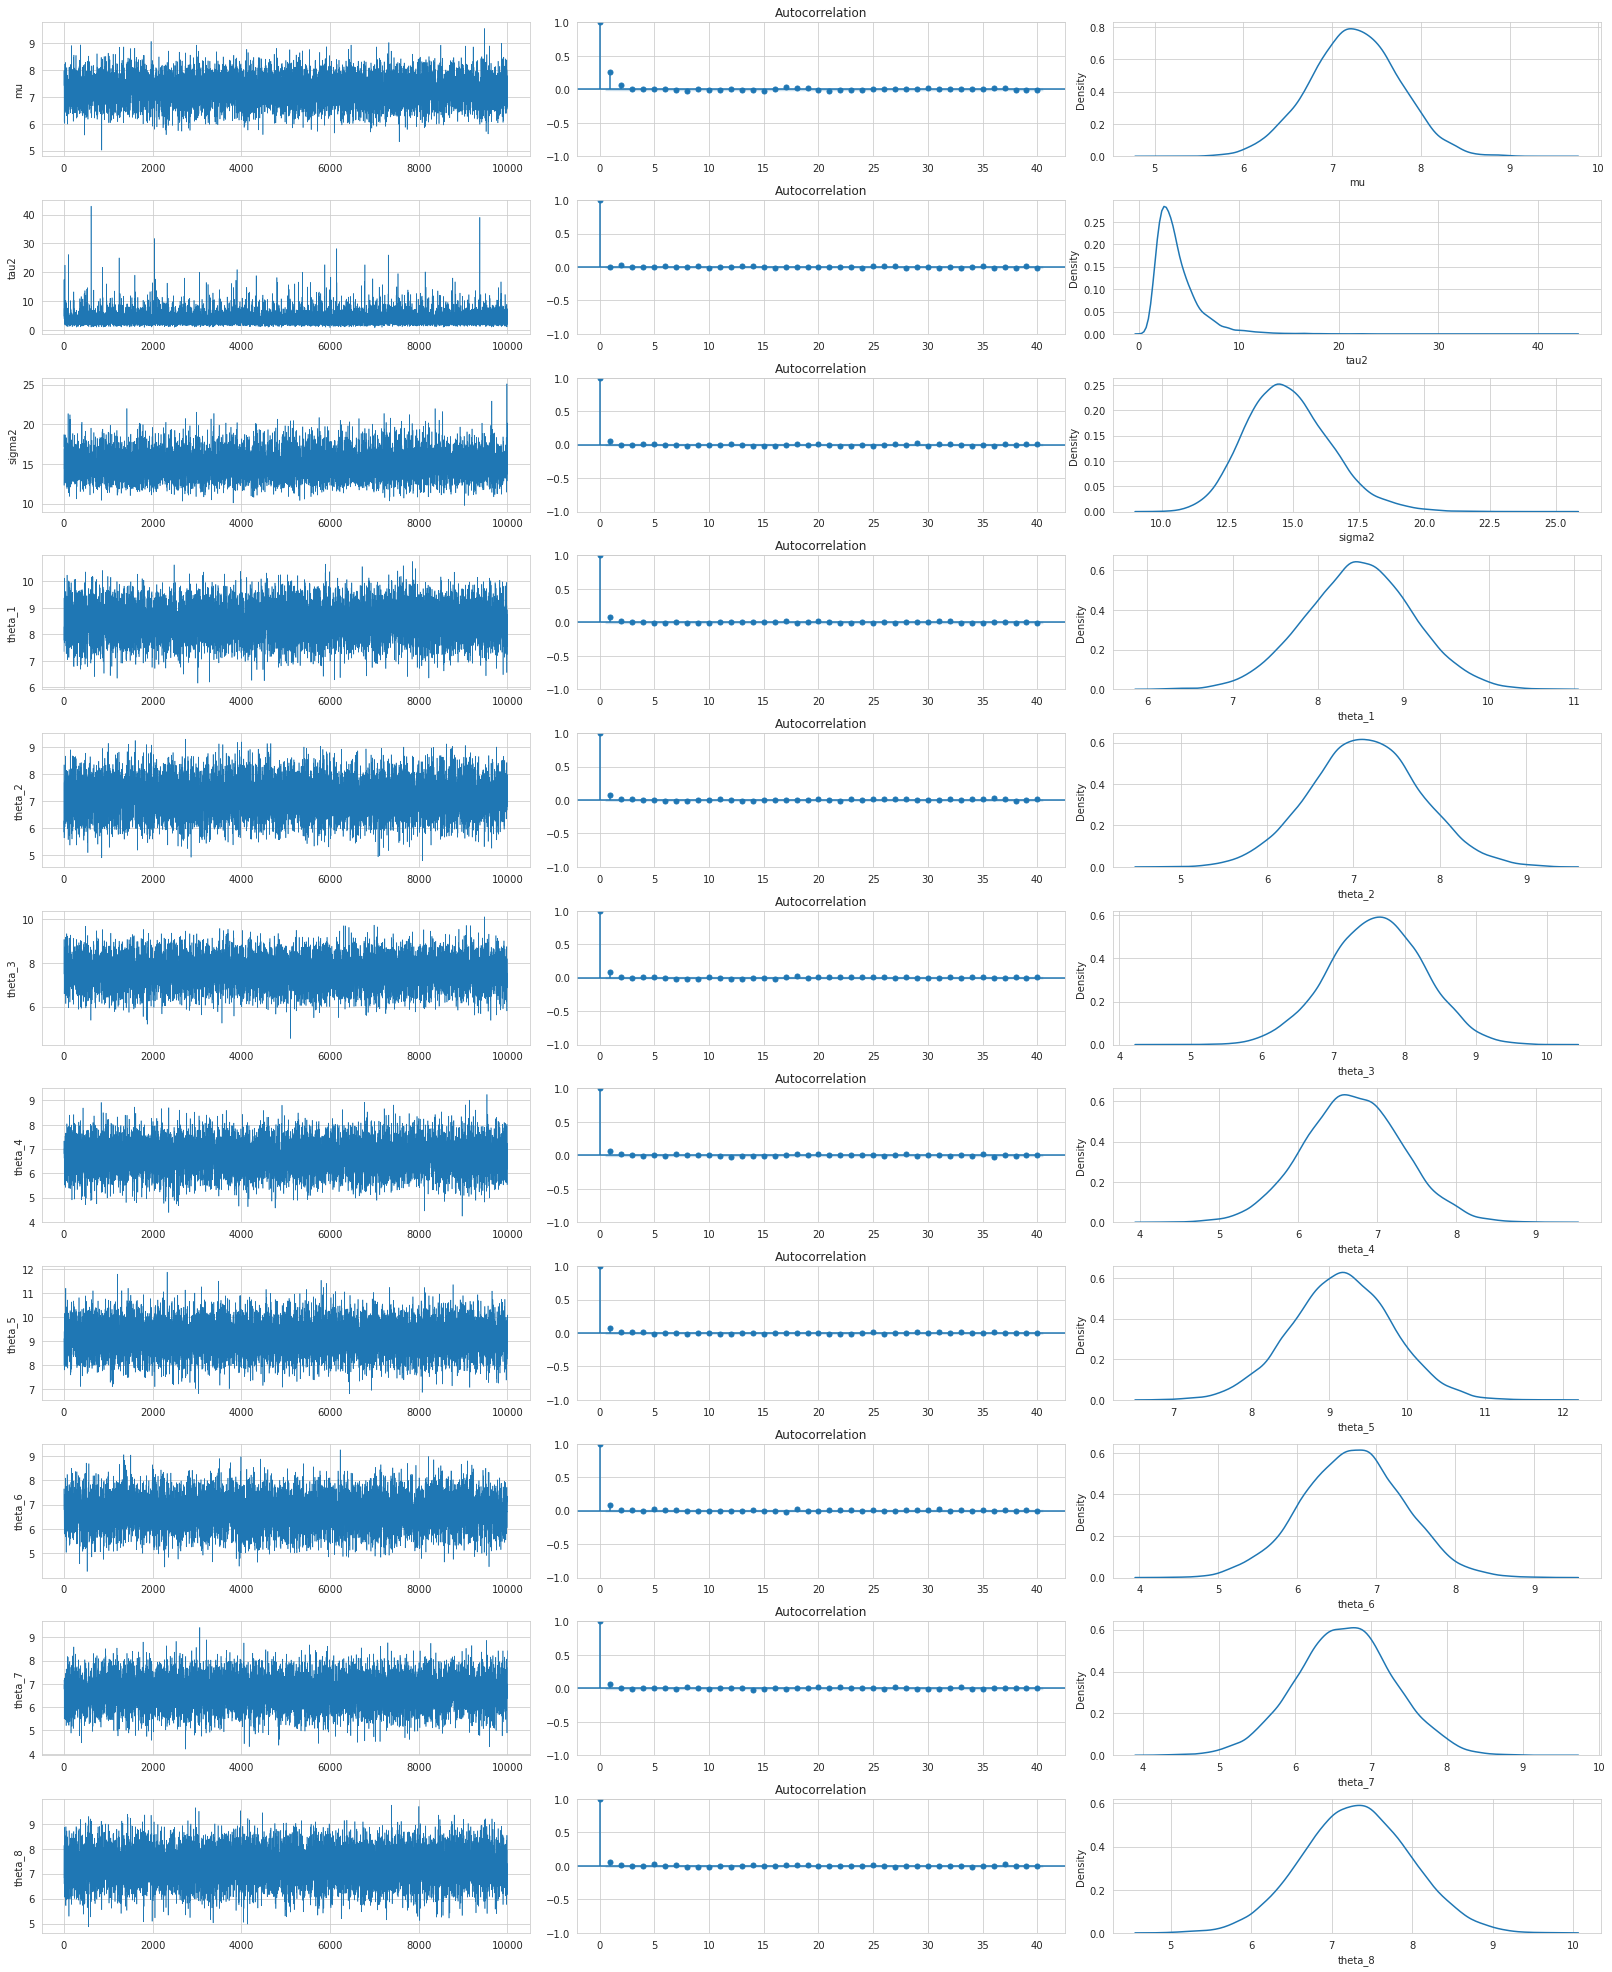
\includegraphics[width=1.0\textwidth]{3.a.png}
  \captionsetup{justification=centering}
  \caption{MCMC Diagnostics}
\end{figure*}

\newpage
\paragraph{(b) Posterior Statistics}
Here are some statistics and prior and posterior comparisons.
\begin{itemize}
    \item $\mu$ posterior mean is 7.25 and 95\% CI $[6.254, 8.221]$
    \item $\tau^2$ posterior mean is 3.85 and 95\% CI $[1.422, 9.800]$
    \item $\sigma^2$ posterior mean is 14.84 and 95\% CI $[11.988, 18.393]$
\end{itemize}
\begin{figure*}[!h]
  \centering
  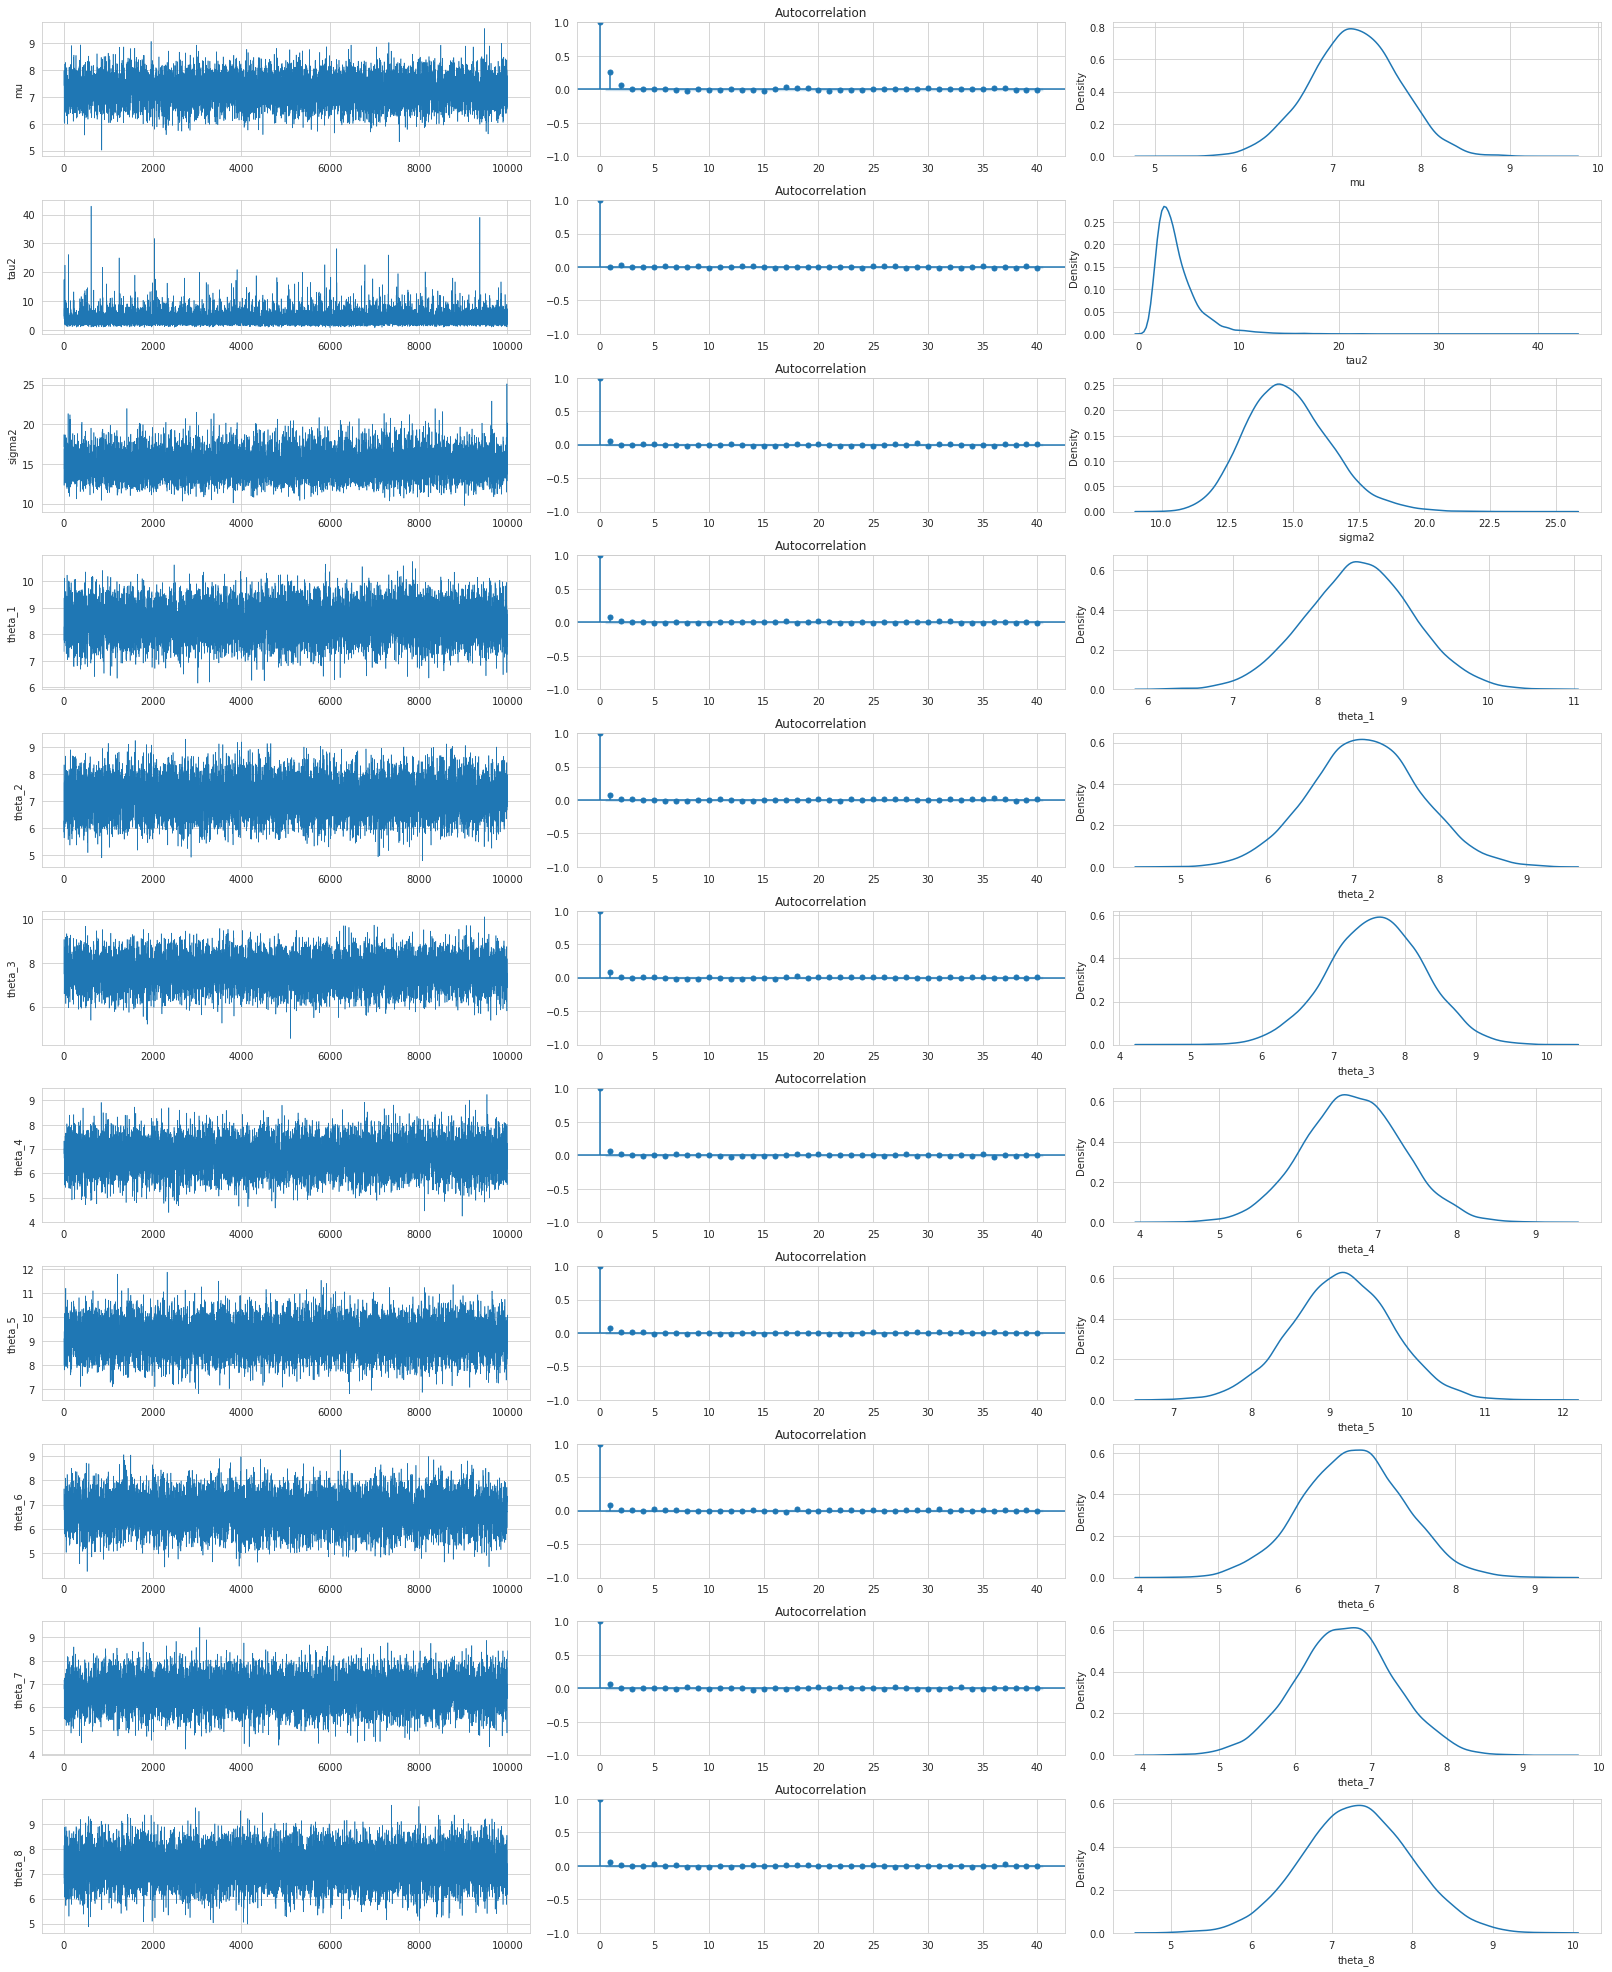
\includegraphics[width=1.0\textwidth]{3.a.png}
  \captionsetup{justification=centering}
  \caption{Posteriors of three priors}
\end{figure*}


\end{document}